\section{Description of Classic Q-learning Algorithm}
We introduce the classic Q-learning algorithm in both offline and online settings.
\paragraph{Q-learning}
Q-learning is a classic value-based RL algorithm, which iteratively applies the Bellman optimal operator to train the Q-function, formally written as $\mathcal{B}^*Q(s,a)=r(s,a)+\gamma \mathbb{E}_{s^\prime\sim P(\cdot|s,a)}\left[\max_a^\prime Q(s^\prime,a^\prime)\right]$. After the optimal Q-function $Q^*$ learned, then the optimal action policy respect to the $Q^*$ is given as: $\pi^*(\cdot|s)=\arg\max_a Q^*(s,a)$. DQN \citep{mnih2013playing} is a well-known Q-learning algorithm, which can process various classes of the state information such as image and language, which learns a deep neural network $Q^\theta(s,a)\approx Q^*(s,a)$ to approximate $Q^*(s,a)$ and uses TD-learning to iteratively update the Q network, the loss function for the $i$-the iteration is given as: 
\begin{equation}
\mathcal{L}_i(\theta)=\mathbb{E}_{(s,a,s^\prime)\sim \mathcal{D}}\left[(Q^{\theta_i}(s,a)-y_i)^2\right],
\end{equation}
where $\mathcal{D}$ is the reply buffer, $y_i=\mathcal{B}^*Q^{\theta_{i-1}}(s,a)=r(s,a)+\gamma \max_{a^\prime\in \mathcal{A}} Q^{\theta_{i-1}}(s^\prime,a^\prime)$. $\theta_{i-1}$ is the learned parameters of the last iteration and is frozen during the gradient descent for optimizing the loss function $\mathcal{L}_i$.
\paragraph{Conservative Q-learning}
CQL \citep{kumar2020conservative} framework is designed for offline reinforcement learning, where only offline data is available, but no further online exploration is accessible. Different from traditional Q-learning, CQL introduces an additional regularization term on top of the standard DQN framework or actor-critic framework(such as SAC \citep{haarnoja2018soft}), ensuring that the learned Q-function lower-bounds the actual value. The lower-bounded Q-values help mitigate the overestimation problem commonly encountered with out-of-distribution (OOD) state-action pairs. The CQL loss on the top of value-based DQN is given as:
\begin{equation}
\mathcal{L}_i(\theta)=\beta\mathbb{E}_{(s,a)\sim \mathcal{D}}\left[\log \sum_{a^\prime\in \mathcal{A}} \exp(Q^{\theta_i}(s,a^\prime))-Q^{\theta_i}(s,a)\right]+\frac{1}{2}\mathbb{E}_{(s,a,s^\prime)\sim \mathcal{D}} \left[(Q^{\theta_i}(s,a)-y_i)^2\right],
\end{equation}
where $y_i=r(s,a)+\gamma \max_{a^\prime} Q^{\theta_{i-1}}(s^\prime,a^\prime)$ and $\beta$ is a hyper-parameter.


\section{Proofs}

\subsection{Probabilistic Inference Derivation}\label{appendix: probabilistic}
In this section, we derive the detailed formulation for probabilistic inference for using LLM as a prior. This includes the policy-based method where we learn a parametrized policy function and the value-based method where we directly perform posterior inference.

\paragraph{Variational Inference}
 Assume that we have the optimality variable $\mathcal{O}$ indicating the quality of a trajectory $\tau = \{s_0, a_0, r_0, s_{1}, ..., s_n \}, p(\tau) = p(s_0)\prod_t p(a_t|s_t)p(s_{t+1}|s_t, a_t)$. The likelihood function with temperature parameter $\alpha$ can be written as:
\begin{equation}
    p(\mathcal{O}=1|\tau) = \exp \left(\sum_t \gamma^tr_t/\alpha \right)
\end{equation}
Our goal is to maximize the optimal marginal distribution formulated as follows:
\begin{equation}
\begin{aligned}
    p(\mathcal{O}=1) & =  \int p(\mathcal{O}=1, \tau) d\tau \\
    & = \int q(\tau) \frac{p(\mathcal{O}=1|\tau)p(\tau)}{q(\tau)} d\tau 
\end{aligned}
\end{equation}
where $q(\tau)$ is a parametrized variational distribution. Then, our variational inference objective can be written as:
\begin{equation}
\begin{aligned}
\log p(\mathcal{O}=1) & \geq \int q(\tau) \log \left[p(\mathcal{O}=1|\tau) \frac{p(\tau)}{q(\tau)} \right] d\tau \\
& = \mathbb{E}_{q(\tau)}\left[\log p(\mathcal{O}=1|\tau) \right] - \textbf{KL}\left[q(\tau) | p(\tau)\right] \\
& = \textbf{ELBO}
\end{aligned}
\end{equation}
In the context of language models, we define prior $p(\tau)$ as trajectory distribution generated through a fixed LLM denoted as:
\begin{equation}\label{eq: llm prior}
    p_{LLM}(\tau) = p(s_0)\prod_t p_{LLM}(a_t|s_t)p(s_{t+1}|s_t, a_t)
\end{equation}
where $p_{LLM}(a_t|s_t)$ is the probability likelihood of the generated output $a_t$ given input text $s_t$. The variational distribution $q(\tau)$ can also be decomposed in the same way as:
\begin{equation}
    q(\tau) = p(s_0)\prod_t \pi_{\theta}(a_t|s_t)p(s_{t+1}|s_t, a_t)
\end{equation}
where the parametrized policy function $\pi_{\theta}$ can be a learnable language model with parameter $\theta$. Substituting these factorizations back to ELBO we have the step-wise objective function written as:
\begin{equation}
    -\mathcal{L} = \sum_{t} \mathbb{E}_{\pi_{\theta}}\left[\gamma^t r_t \right] - \alpha \textbf{KL}\left[ \pi_{\theta}(a_t|s_t) \| p_{LLM}(a_t|s_t) \right]
\end{equation}
\begin{equation}
    \pi^{*} = \argmin_{\theta} \mathcal{L}
\end{equation}



\paragraph{Direct Posterior Inference} Instead of learning a parametrized policy which might involve fine-tuning a language model, we can also try directly sampling from the posterior distribution formulated as:
\begin{equation}
\begin{aligned}
     p(\tau|\mathcal{O}=1) & = \frac{p(\mathcal{O}=1|\tau)p(\tau)}{p(\mathcal{O}=1)}\\
     & \propto p(\mathcal{O}=1|\tau)p(\tau) \\
     & = \prod_{t}p(\mathcal{O}_t=1|s_t, a_t)p_{LLM}(a_t|s_t)p(s_{t+1}|s_{t}, a_t)
\end{aligned}
\end{equation}
in which we define $p(\tau)$ as in Equation \ref{eq: llm prior}. According to Control-as-Inference framework proposed by \cite{levine2018reinforcement}, we can formulate posterior inference as Soft Q-Learning where Q-values are updated using a modified soft Bellman equation:
\begin{equation}
\begin{aligned}
    Q^{\pi}(s_t, a_t) = r(s_t, a_t) + \gamma \mathbb{E}_{s_{t+1}\sim p(\cdot|s_t, a_t)}\left[V(s_{t+1}) \right] \\
    V(s_t) = \log\int \exp (Q(s_t, a_t)/\alpha) da_t
\end{aligned}
\end{equation}
and the policy can be defined as a softmax function over the Q-values: $\pi(a|s) = \exp(Q^{\pi}(s,a)/\alpha) / \int_{a^{'}} \exp(Q^{\pi}(s,a^{'})/\alpha) da^{'}$, ensuring that actions with higher Q-values are more likely to be chosen. In our paper, however, due to the enormously large space of (textual) state-action pair, we also apply sampling approximation methods. Specifically, we leverage similar ideas from \cite{fourati2024stochastic} which sample a random subset of actions from the complete action space and seek the optimal within this subset. In our case, we rely on a fixed LLM to provide such action subspace and can further narrow down the space through repeated sampling (\cite{brown2024large}):
% through repeated sampling (\cite{brown2024large}):
\begin{equation}
\begin{aligned}
    \pi(a|s) & = \frac{\mathbf{1}_{a \in p_{LLM}(\cdot|s) } \cdot \exp\left(Q^{\pi}(s, a)/\alpha\right)}{
    \int_{a^{'}} \mathbf{1}_{a \in p_{LLM}(\cdot|s) } \cdot \exp\left(Q^{\pi}(s, a^{'})/\alpha\right) da^{'}
    } \\
    & \approx \mathbf{1}_{a\in\{a^i\}} \cdot \frac{1}{N} \frac{\exp(Q^{\pi}(s, a^{i})/\alpha)}{\sum_{i}\exp(Q^{\pi}(s, a^{i})/\alpha)}, a^i \sim p_{LLM}(a|s)
\end{aligned}
\end{equation}
This means we restrict the Bellman backup to a specific action subspace that can potentially provide a refined set of actions based on context, largely reducing computational complexity and focusing on more relevant actions.





% and aim to learn a step-wise scoring function $f(s,a)$ taking state-action pair in textual MDP and approximating the likelihood distribution $p(\mathcal{O}=1|\tau)$.



\subsection{Proof of Proposition \ref{proposition}}
\propsa*
\begin{proof}
The proof mainly follows the \citep{li2024q}. Denote the above sampling strategy indeed follows a distribution $q$, and for each action $a$, the probability of $a$ is sampled from the distribution $q$ is given by:
\begin{equation}
    %\lim_{k\rightarrow\infty} ()
    \begin{aligned}
            q(a|s_t)&=\mathbb{E}_{\{a_1,\cdots,a_k\}\sim p_\text{LLM}(\cdot|s)}\left[\sum_{i=1}^k \mathbb{I}(a_i=a) \frac{\exp( Q^\theta(s_t,a_i)/\alpha)}{\sum_{j=1}^k \exp( Q^\theta(s_t,a_j)/\alpha)}\right]\\
            &=\mathbb{E}_{\{a_1,\cdots,a_k\}\sim p_\text{LLM}(\cdot|s)}\left[ \frac{\sum_{i=1}^k \mathbb{I}(a_i=a)}{\sum_{j=1}^k \exp( Q^\theta(s_t,a_j)/\alpha)}\right]\exp( Q^\theta(s_t,a)/\alpha)\\
            &=\mathbb{E}_{\{a_1,\cdots,a_k\}\sim p_\text{LLM}(\cdot|s_t)}\left[ \frac{\frac{1}{k}\sum_{i=1}^k \mathbb{I}(a_i=a)}{\frac{1}{k}\sum_{j=1}^k \exp( Q^\theta(s_t,a_j)/\alpha)}\right]\exp( Q^\theta(s_t,a)/\alpha)\\
    \end{aligned}
\end{equation}
According to the Law of Large Numbers, when $k\rightarrow \infty$, we have:
\begin{equation}
\begin{aligned}
        \lim_{k\rightarrow\infty} q(a|s_t)&= \lim_{k\rightarrow\infty} \mathbb{E}_{\{a_1,\cdots,a_k\}\sim p_\text{LLM}(\cdot|s_t)}\left[ \frac{\frac{1}{k}\sum_{i=1}^k \mathbb{I}(a_i=a)}{\frac{1}{k}\sum_{j=1}^k \exp( Q^\theta(s_t,a_j)/\alpha)}\right]\exp( Q^\theta(s_t,a)/\alpha)\\
        &= \lim_{k\rightarrow\infty} \mathbb{E}_{\{a_1,\cdots,a_k\}\sim p_\text{LLM}(\cdot|s_t)}\left[ \frac{p_\text{LLM}(a|s_t)}{\mathbb{E}_{a_j \sim p_\text{LLM}(\cdot|s_t)} \exp( Q^\theta(s_t,a_j)/\alpha)}\right]\exp( Q^\theta(s_t,a)/\alpha)\\
        &= p_\text{LLM}(a|s_t)\frac{\exp( Q^\theta(s,a)/\alpha)}{\mathbb{E}_{a_j \sim p_\text{LLM}(\cdot|s)} \exp( Q^\theta(s,a_j)/\alpha)}
\end{aligned}
\end{equation}
Following the proof process from the Appendix A.1. in \cite{rafailov2023direct}, we have:
\begin{equation}
\label{dpo}
    \arg\max _\pi \mathbb{E}_{\pi(a|s_t)} [Q^\theta(s_t,a)]-\alpha \text{KL}\left(\pi(\cdot|s_t)\|p_\text{LLM}(\cdot|s_t)\right)=p_\text{LLM}(a|s_t)\frac{\exp( Q^\theta(s,a)/\alpha)}{\mathbb{E}_{a_j \sim p_\text{LLM}(\cdot|s)} \exp( Q^\theta(s,a_j)/\alpha)}
\end{equation}
\end{proof}

Additionally, as shown in Sec. \ref{sec: method}, the variational inference approach learns the optimal policy $\pi$ by maximising:
\begin{equation}
\label{variation_appen}
%\arg\max_\pi \mathcal{J}(\pi) = 
\arg\max_\pi \sum_t  \mathbb{E}_\pi\left[\gamma^t r_t\right] - \alpha \, \text{KL}(\pi(a|s_t) \| p_{\text{LLM}}(a|s_t)).
\end{equation}
Introducing the occupancy measure $\rho$, $\rho(s)=\frac{1}{1-\gamma}\sum_{t=0}^\infty [\gamma^t \mathbb{P}(s_t=s|a\sim \pi)]$, we have the following form objective respected to the Q-function
\begin{equation}
\label{optq}
\arg\max_\pi \mathbb{E}_{\rho(s)}[\mathbb{E}_{a\sim\pi}[Q^\pi(s,a)]-\alpha \text{KL}(\pi(a|s_t) \| p_{\text{LLM}}(a|s_t))]
\end{equation}
Combining Equations \ref{dpo} and \ref{optq}, we find that the variational inference approach and the direct posterior sampling yield similar solutions.
\section{Additional Experiment Details}
\subsection{Environments}

We consider three environments:
\newline\textbf{ALFWorld} %This game connects the text-based world of TextWorld with the parallel embodied worlds in the ALFRED dataset. 
 We consider two classes of ALFWorld tasks: ALFWorld(pick) and ALFWorld(examine). For ALFWorld (Pick), we evaluate the online training baselines on 28 tasks, such as "put the cellphone on the armchair," and test the generalization ability on 26 unseen tasks. For ALFWorld (Examine), we use 11 tasks, such as "examine the laptop with the desk lamp." There are no auxiliary rewards, except for a reward of $1.0$ for reaching the final goal. 
\newline\textbf{Overcooked} We use the partially observed text overcooked game; the observation describes the position of visible items, and the agent should take a sequence of actions to deliver a dish. We consider two overcooked tasks: Overcooked(Tomato), deliver a dish of chopped tomato; Overcooked(Salad), deliver a salad containing chopped tomato and lettuce. The maximum possible action space is $8$. Besides the reward of $1$ for successfully delivering a dish, the textual Overcooked environment from \cite{tantrue} also provides dense reward signals. The reward shaping is as follows: 0.2 for correctly chopping an ingredient, 1 terminal reward for successfully delivering the correct dish, $-0.1$ for delivering any incorrect item, and $-0.001$ for each time step.
\newline\textbf{Frozen Lake} is a grid world game; the agent should move to the goal position while avoiding full into holes. There are four admissible actions: up, down, right, and left. The agent will receive a reward of $1$ for reaching the final goal and a penalty of $-1$ for falling into holes. The maximum steps for these three tasks are shown in Table \ref{tab:horizon}.
\begin{table}[]
    \centering
    \begin{tabular}{c|ccccc}
    \hline
         & ALFWorld(Pick) &ALFWolrd(Examine) &Cook(Tomato)&Cook(Salad) &Frozen Lake  \\
         \hline
         Horizon& 60&60&30&50&20 \\
         \hline
    \end{tabular}
    \caption{Maximize horizon of environments. }
    \label{tab:horizon}
\end{table}

\subsection{LLM prior implementation}
There are two ways to sample an action $a$ from the LLM prior $p_{\text{LLM}}(\cdot | s_t)$. First, since the state and action can be described as text, and assuming the action $a$ consists of $k$ tokens, the probability of the LLM generating action $a$ is given by $p(a | s_t) = \prod_{i=1}^k p_{\text{LLM}}(a_i | s_t, a_{<i})$. Based on this probability, the first type of LLM prior computes a distribution over actions, denoted as $p_{\text{LLM}}^{\text{dist}}(a | s_t) = \frac{\exp p(a | s_t)}{\sum_{a^\prime} \exp p(a^\prime | s_t)}$. In contrast, the second approach involves sampling a free-form output from the LLM, which is then mapped to an executable action via a simple rule-based projection $\mathcal{P}$. We denote this LLM prior, which relies on mapping the LLM's output, as $p_{\text{LLM}}^{\text{map}}$, where $a \sim p_{\text{LLM}}^{\text{map}}(\cdot | s_t) \leftrightarrow o \sim \text{LLM}(\cdot | s_t), a = \mathcal{P}(o)$.


%The KL-divergence encourages the learned policy \(\pi\) to stay close to the powerful LLM prior, which is often powerful. In practice, the cumulative reward is straightforward to compute by rolling out an entire trajectory. For computing the KL-divergence, LLM-based RL approaches \cite{carta2023grounding, wen2024entropy} can either: 1) directly compute the distribution over action in the form of $p_{\text{LLM}}^{\text{dist}}$, or 2) simplify the KL computation by focusing solely on a sample from \(p^\text{map}_{\text{LLM}}(a|s_t)\), where actions generated with high probability by the LLM prior are more likely to be selected \cite{zhang2024can}.


We observed a performance gap between these two types of LLM action priors. For instance, in the ALFWorld pick \& place task, $p_{\text{LLM}}^{\text{map}}$ achieved a winning rate of $19\%$, while $p_{\text{LLM}}^{\text{dist}}$ failed, with a winning rate of $0\%$, both using the LLM Qwen1.5-7B. Therefore, in this work, we implement $p_{\text{LLM}}^{\text{map}}$ as the LLM prior for thoughtfully exploiting the power of the LLM in SDM tasks, which we denote as $p_{\text{LLM}}$ for simplicity.
Examples of LLM's output is given as:
\begin{tcolorbox}[title={For ALFWorld(Pick) from Qwen-1.5 7B}]
    
\textbf{Input:}
Current observation:You are in the middle of a room. Looking quickly around you, you see a armchair 1, a bed 1, a diningtable 1, a drawer 2, a drawer 1, a garbagecan 1, a sidetable 2, and a sidetable 1.

Your task is to: put some cellphone on armchair.. You are allowed to take the following actions: go to armchair 1, go to bed 1, go to diningtable 1, go to drawer 1, go to drawer 2, go to garbagecan 1, go to sidetable 1, go to sidetable 2, inventory, look.
Please select an action from the admissible actions. 

\textbf{Output:} 
1: take cd 2 from sidetable 2 , 

2: Open drawer 2 Result: You open door, 

3: look Description: You look around the room., 

4: look > Current observation:You arrive at loc, 

5: open drawer 2 Loc 8: You

\end{tcolorbox}
\subsection{Hyper-parameters}
Our algorithms are trained on one machine with $2$ 40G A100. based on Pytorch-GPU 2.1 and cuda12.4. Table \ref{tab:tomato},\ref{tab:salad},\ref{tab:lake},\ref{tab:pick},\ref{tab:exam} reports the main hyper-parameters of our algorithms. For all CQL-based algorithms, we set the hyperparameter $\beta$ for regulating the Q-values, as shown in \eq \ref{cql_loss}, as $5.0$.
\paragraph{Offline Datasets}
The composition of offline datasets is shown in Table \ref{tab:offline_data}, which reports the number of $(s,a,s^\prime)$ examples.

\begin{table}[]
    \caption{The hyperparameters on ALFWorld(Pick)}
    \centering
    \begin{tabular}{cccccccc}
    \hline
    Baselines & Learning Rate & Epochs & Batch Size & Update Frequency& LLM &$\alpha$\\
    \hline
        DQN-Prior & 5e-4& 4&128&5&/ &0.01  \\
        CQL-Prior & 5e-4& 4&128&5  &/ &0.01 \\
        GFlan-Prior  & 1e-4& 16&64&16&Flan-T5 Small&0.01  \\
    \hline
        \end{tabular}
    \label{tab:paralake}
\end{table}
\begin{table}[]
    \caption{The hyperparameters on ALFWorld(Examine)}
    \centering
    \begin{tabular}{cccccccc}
    \hline
    Baselines & Learning Rate & Epochs & Batch Size & Update Frequency& LLM &$\alpha$\\
    \hline
        DQN-Prior & 5e-4& 4&128&10&/ &0.01  \\
        CQL-Prior & 5e-4& 4&128&10  &/ &0.01 \\
        GFlan-Prior  & 1e-4& 16&64&16&Flan-T5 Small&0.01  \\
    \hline
        \end{tabular}
    \label{tab:paralake}
\end{table}
\begin{table}[]
    \caption{The hyperparameters on Overcooked(Tomato
    )}
    \centering
    \begin{tabular}{cccccccc}
    \hline
    Baselines & Learning Rate  & Batch Size & Update Frequency& LLM &$\alpha$\\
    \hline
        DQN-Prior & 5e-4&128&5&/ &0.1  \\
        CQL-Prior & 5e-4&128&5  &/ &0.1 \\
        GFlan-Prior  & 1e-4&64&16&Flan-T5 Small&0.1  \\
    \hline
        \end{tabular}
    \label{tab:tomato}
\end{table}
\begin{table}[]
    \caption{The hyperparameters on Overcooked(Salad)}
    \centering
    \begin{tabular}{cccccccc}
    \hline
    Baselines & Learning Rate  & Batch Size & Update Frequency& LLM &$\alpha$\\
    \hline
        DQN-Prior & 5e-4&128&5&/ &0.1  \\
        CQL-Prior & 5e-4&128&5  &/ &0.1 \\
        GFlan-Prior  & 1e-4&64&16&Flan-T5 Small&0.1  \\
    \hline
        \end{tabular}
    \label{tab:salad}
\end{table}
\begin{table}[]
    \caption{The hyperparameters on Frozen Lake}
    \centering
    \begin{tabular}{cccccccc}
    \hline
    Baselines & Learning Rate  & Batch Size & Update Frequency& LLM &$\alpha$\\
    \hline
        DQN-Prior & 5e-4& 128&5&/ &0.1  \\
        %CQL-Prior & 5e-4& 4&128&5  &/ &0.1 \\
        %GFlan-Prior  & 1e-4& 16&128&64&Flan-T5 Small&0.1  \\
    \hline
        \end{tabular}
    \label{tab:lake}
\end{table}
\begin{table}[]
    \caption{The hyperparameters on ALFWorld(Pick)}
    \centering
    \begin{tabular}{cccccccc}
    \hline
    Baselines & Learning Rate  & Batch Size & Update Frequency& LLM &$\alpha$\\
    \hline
        DQN-Prior & 5e-4&128&10&/ &0.01  \\
        CQL-Prior & 5e-4&128&10  &/ &0.01 \\
        GFlan-Prior  & 1e-4&64&16&Flan-T5 Small&0.01  \\
    \hline
        \end{tabular}
    \label{tab:pick}
\end{table}
\begin{table}[]
    \caption{The hyperparameters on ALFWorld(Examine)}
    \centering
    \begin{tabular}{cccccccc}
    \hline
    Baselines & Learning Rate  & Batch Size & Update Frequency& LLM &$\alpha$\\
    \hline
        DQN-Prior & 5e-4&128&10&/ &0.01  \\
        CQL-Prior & 5e-4&128&10  &/ &0.01 \\
        GFlan-Prior  & 1e-4&64&16&Flan-T5 Small&0.01  \\
    \hline
        \end{tabular}
    \label{tab:exam}
\end{table}
\begin{table}[]
    \centering
    \begin{tabular}{c|ccc}
    \hline
         Dataset & Total Examples & Good Examples & Bad Examples  \\
         \hline
         ALFWorld(Pick)&6572&6572&0 \\
         Salad(1000)&1186&574&612\\
         Salad(4000)&3892&2209&1683\\
         Salad(8000) &7571&4224&3347\\
         Salad(12000)&11939&4004&7935\\
           Salad(24000)&23869&7191&16678\\
\hline
    \end{tabular}
    \caption{The composition of the offline dataset}
    \label{tab:offline_data}
\end{table}
\subsection{Additional Results}
\begin{figure*}[t!]
%  \vspace{-0.5em}
	\centering
 % \includegraphics[width=1.0 \linewidth]{fig/legendablation.pdf}
	{
 
%
\includegraphics[width=0.35 \linewidth]{fig/legendbaselineprior_policy.pdf}
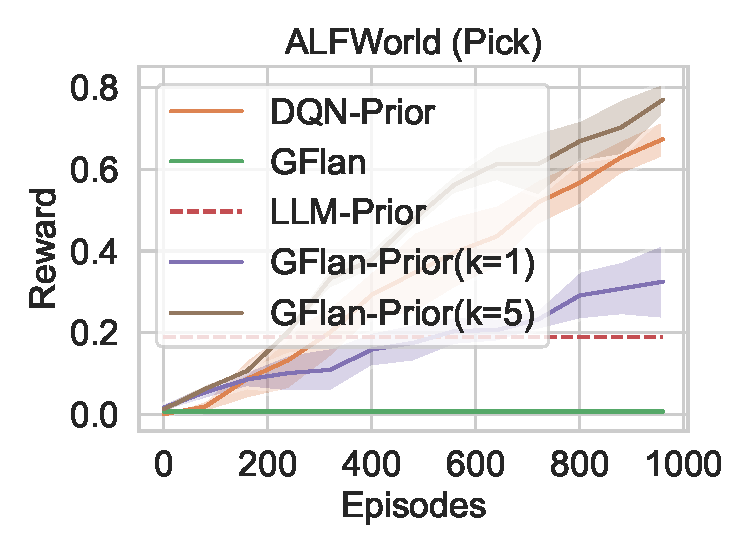
\includegraphics[width=0.28 \linewidth]{fig/train_curve_alf_pick_ab.pdf}
    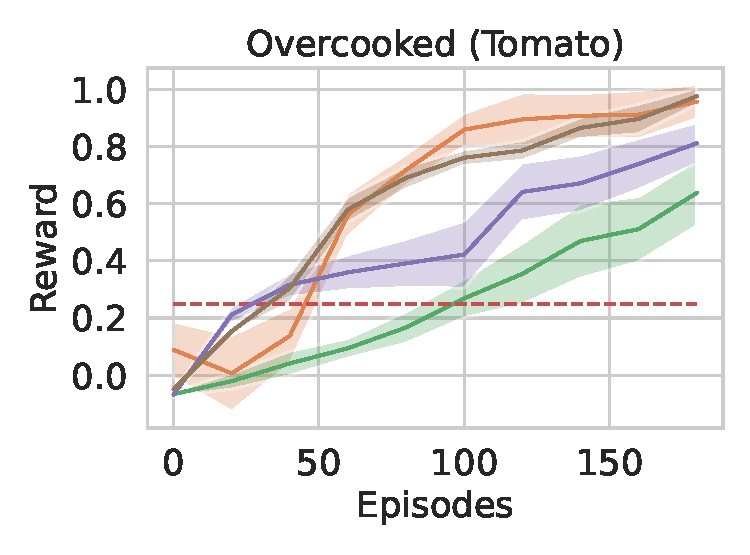
\includegraphics[width=0.28 \linewidth]{fig/train_curve_overcooked_ab.pdf}
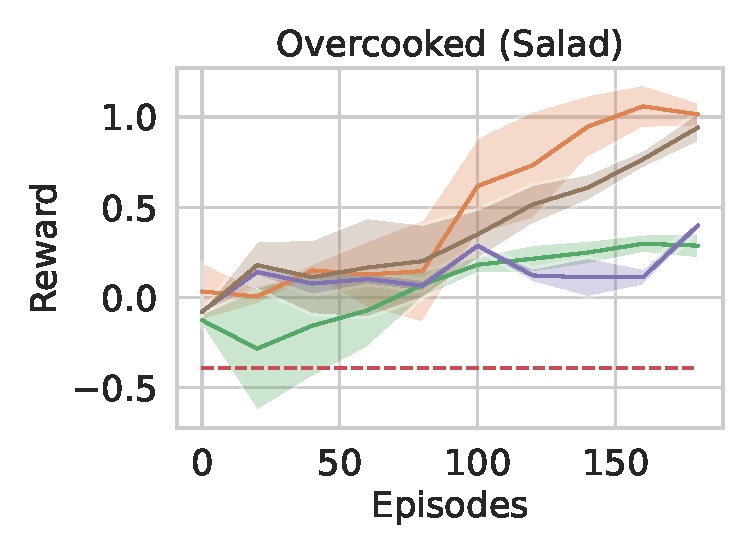
\includegraphics[width=0.28 \linewidth]{fig/train_curve_overcooked_lettuce_ab.pdf}
     }
    
    \caption{The ablation of the number of action proposals $k$ used for approximating KL divergence between the required action policy and the LLM prior action distribution.}%} 
\label{fig:policy_base_k}
\end{figure*}

\paragraph{Additional ablation on $k$ for GFlan-Prior} As shown in \fig \ref{fig:policy_base_k}, when we sample $k=5$ action proposals from the LLM to approximate the KL divergence, it performs better than when using $k=1$. This is because, with more proposals, the optimal action is more likely to be included in the subset, thus better guiding the action policy.

\section{Additional Related Works}\label{sec: extra related works}
\paragraph{Value-based Inference of LLM} Not limited to the pre-training phase, it has been recently investigated how scaling law applies at inference time for LLM. This is often referred to as searching over an enormously large output space with guidance from value estimation. For example, the naive case is beam search (citation) which selects the top K possible sequence based on cumulative probabilities as opposed to greedy search. The value estimate here is the likelihood of the sentence as predicted by the language model. \citep{wang2022self} propose CoT-SC, which searches over reasoning paths and selects the most frequent answer. Tree-of-Thought (ToT, \citep{yao2023tree}) adopts depth/breadth-first search. \citep{hao2023reasoning} introduce Reasoning-via-Planning (RAP) which uses Monte-Carlo Tree Search and value estimate from prompting LLM. TS-LLM designed by \citep{feng2023alphazero} guides MCTS with a learned value function conditioned on state and a learned Outcome-supervised Reward Model (ORM). \citep{li2024q} proposes Q-probing to adapt a pre-trained language model to also maximize a tasks-specific reward function in code generation tasks. Furthermore, recent works investigate Process-supervised Reward Model (PRM, \citep{lightman2023let}) and apply it in LLM inference, \citep{mcaleese2024llm} searches over a step-wise critic model in code reviewing tasks. \citep{wang2024math} learn a PRM in math reasoning and use it for LLM fine-tuning. \citep{snell2024scaling} provides a detailed benchmark of different inference methods. \citep{zhang2024generative} represents the score as the probability of a single text token (e.g. 'Yes' or 'No') under the context and the prompt. Even though our proposed method can be seen as an example of value-based inference, we focus on a different perspective where we investigate how LLM helps conventional value-based reinforcement learning algorithms in complex environments. More discussion can be found in Section \ref{sec: method}.

\iffalse
\section{Reproducibility Statement}
We have provided a detailed description of the algorithm and reported the key hyperparameters and LLM configurations. We are committed to making our code publicly available upon acceptance of the paper.
\fi